\lecture{2010-01-27}

\begin{itemize}
	\item anschaulich: Arbeit, die verrichtet wird \equals\ Fläche unter dem Kraftverlauf
	\item allgemeine Maßtheorie -- Integralbegriffe: 
	\begin{itemize}
		\item deterministisch: Riemann-, Lebesgue-Integral
		\item stochastisch: It\={o}-, Stratonovich-Kalkül
	\end{itemize}
\end{itemize}

\minisec{Voraussetzung}
Gegeben sei eine \emph{beschränkte} Funktion \( f:[a,b]\rightarrow \mathbb{R} \), d. h. es existiert \(  m, M \in \mathbb{R} \) so dass \( m \leq f(x) \leq M \).

\begin{note}
	Wäre \( f \) stetig (oder differenzierbar), dann wäre f sowieso beschränkt, da f auf einem abgeschlossenem Interval \( [a,b] \) definiert ist.
\end{note}

\begin{center}
    \begin{tikzpicture}[]
		\draw[->,semithick] (-0.5,0) -- (11,0) node[below]{x};
		\draw[->,semithick] (0,-0.5) -- (0,3.5) node[left]{y};
		
		\draw (-2pt,1) -- (2pt,1) node[left] {\(m\)};
		\draw (-2pt,2.7182) -- (2pt,2.7182) node[left] {\(M\)};

		\draw[domain=1:3] plot [id=log_ln, samples=100] function { log(x) + 1 };
		\draw [dash pattern=on 1pt off 1pt] (1,0)-- (1,1);
		\draw [dash pattern=on 1pt off 1pt] (3,0)-- (3,2.0986);
		\draw (1,2pt) -- (1,-2pt) node[below] {\(\underbrace{a}_{=x_0}\)};
		
		\draw[domain=3:5] plot [id=efunk, samples=100] function { exp((x-3)/2) };
		\draw [dash pattern=on 1pt off 1pt] (4,0)-- (4,1.6487);
		\draw [dash pattern=on 1pt off 1pt] (5,0)-- (5,2.7182);
		\draw (3,2pt) -- (3,-2pt) node[below] {\(x_1\)};
		\draw (4,2pt) -- (4,-2pt) node[below] {\(x_2\)};
		\draw (5,2pt) -- (5,-2pt) node[below] {\(x_3\)};
		
		\draw[domain=7:8] plot [id=const, samples=100] function { exp(1) };
		\draw [dash pattern=on 1pt off 1pt] (7,0)-- (7,2.7182);
		\draw [dash pattern=on 1pt off 1pt] (8,0)-- (8,2.7182);
		\draw (7,2pt) -- (7,-2pt) node[below] {\(x_4\)};
		\draw (8,2pt) -- (8,-2pt) node[below] {\(x_5\)};
		
		\draw[domain=8:10] plot [id=einsdurch, samples=100] function { exp(1)/(x-7) };
		\draw [dash pattern=on 1pt off 1pt] (10,0)-- (10,0.9060);
		\draw (10,2pt) -- (10,-2pt) node[below] {\(\underbrace{b}_{=x_b}\)};
		
	\end{tikzpicture}
	\captionof{figure}{erlaubtes \( f(x) \)}
\end{center}

\noindent \( f \) darf Sprünge und Lücken haben -- allerdings nicht zu viele (Bsp.: Signalverarbeitung) \\
pathologisches \( f \): \( f(x) = \begin{cases}1 & x \in \mathbb{Q} \\ 0 & x \in \mathbb{R} \setminus \mathbb{Q}\end{cases} \)

\subsubsection*{Intervallunterteilung (Zerlegung $Z$)}

\begin{align*}
	h &= \frac{b-a}{n} \\
	x_k &= a+k \cdot h \quad k=0,\ldots,n \\
	a &= x_0<x_1<x_2<\ldots<x_n=b 
\end{align*}
Die Stützstellen sind dabei (aus Bequemlichkeit) äquidistant. Betrachtet man nun \(f\) in den Teilintervallen \( [x_{k-1},x_k] \), so gilt aufgrund der Beschränktheit der Funktion: \( m_k \leq f \leq M_k \) auf \( [x_{k-1},x_k] \)
\begin{align*}
	m_k &= \inf f(x) \\
	M_k &= \sup f(x)
\end{align*}

\begin{note}
	Ist \( f \) stetig, gilt im Intervall \( [x_{k-1},x_k] \):
	\begin{align*}
		m_k &= \min f(x) \\
		M_k &= \max f(x)
	\end{align*}	
\end{note}

\begin{definition}[Untersumme von $f$ zur Zerlegung $Z$]
	\[
		\mathcal U(f, Z)= \sum_{k=1}^nm_k(x_k-x_{k-1}) \qquad \text{einbeschriebenes Rechteck}
	\]
\end{definition}


\begin{definition}[Obersumme von $f$ zur Zerlegung $Z$]
	\[
		\mathcal O(f, Z)= \sum_{k=1}^nM_k(x_k-x_{k-1})  \qquad \text{umbeschriebenes Rechteck}
	\]
\end{definition}

\noindent Es gilt: \( \mathcal U(f,Z) \leq \mathcal O(f,Z) \), denn
	\[ \mathcal O(f,Z)- \mathcal U(f,Z)=\sum_{k=1}^n(\underbrace{M_k-m_k}_{\geq0})(\underbrace{x_n-x_{k-1}}_{>0}) \geq 0 \]
\noindent Verfeinerung der Zerlegung liefert die feinere Unterteilung \( Z^\star \):
	\[ \mathcal U(f,Z) \leq \mathcal U(f, Z^\star) \leq \mathcal O(f,Z^\star) \leq \mathcal O(f,Z) \]
\noindent Grenzprozess \( n \rightarrow \infty \): Zerlegungsfolgen \( (Z_s)_{s\in\mathbb{N}} \implies \) 
	\begin{align*}
		\mathcal U &= \sup \mathcal U(f,Z_j) &\text{größte einbeschriebene Rechtecksfläche}\\
		\mathcal O &= \inf \mathcal O(f,Z_j) &\text{kleinste umbeschriebene Rechtecksfläche}
	\end{align*}

\begin{definition}[Integrierbarkeit]
	Sei \( f[a,b] \rightarrow \mathbb{R} \) beschränkt, so gilt
	\begin{align*}
		\mathcal U &= \sup \mathcal U(f,Z_j)\\
		\mathcal O &= \inf \mathcal O(f,Z_j)\\
		\mathcal U &= \mathcal O \implies \text{$f$ ist integrabel}
	\end{align*}
	Die Zahl \( \mathcal U = \mathcal O \) heißt Integral von \( f \) über \( [a,b] \).
\end{definition}

\begin{note}
	\( f \geq 0 \): Integral \equals\ Flächeninhalt
\end{note}

\subsubsection*{Bezeichnung}
\begin{align*}
	f&: \text{ Integrand} \\
	x&: \text{ Integrationsvariable}\\
	a,b&: \text{ untere/obere Integrationsgrenze}\\	
	\int\limits_a^b \,\diff x &:\text{ Integrationssymbol}
\end{align*}

\begin{example}[\mbox{$f(x)=x$ in $[0,b]$}]
	\[
		\int\limits_0^b f(x) \,\diff x = \int\limits_0^b x \,\diff x = I_f = b \cdot b \cdot \frac{1}{2} = \frac{1}{2} \cdot b^2
	\]
\end{example}


\begin{center}
	\definecolor{myblue}{HTML}{92dcec}
    \begin{tikzpicture}[]
		\draw[domain=0:4, fill=myblue] plot [id=easy_func, samples=100] function { x } -- (4,0);
		\draw [dash pattern=on 1pt off 1pt] (4,0)-- (4,4);
		\node at (4.3,2) {$b$};
		\node at (1.8,3) {$f(x)=x$};
		\node at (2.5,1.3) {$I_f$};
		\draw[->,semithick] (-0.5,0) -- (5,0) node[below]{x};
		\draw[->,semithick] (0,-0.5) -- (0,5) node[left]{y};
	\end{tikzpicture}
\end{center}


\subsubsection*{Riemann-Formalismus}
Testfall:
\begin{align*}
	Z_n &= \left\{0,\frac{b}{n},\frac{2b}{n},\ldots,\frac{(n-1)\cdot b}{n}, b\right\} \\
	\quad h &= \frac{b}{n} \quad x_k=h \cdot k \quad k=0,\ldots,n \qquad \text{(äquidistante Stützstellen)} 
\end{align*}

\begin{align*}
	\mathcal U(f,Z_n) 
	&= \sum_{k=1}^n m_k(x_k-x_{k-1}) \\
	&= \sum_{k=1}^n x_{k-1}(x_k-x_{k-1}) \\
	&= \sum_{k=1}^n (k-1)h \cdot h = \left( \frac{b}{n} \right)^2 \sum_{k=1}^n (k-1) \\
	&= \frac{b^2}{n^2} \frac{n}{2}(n-1) = \frac{b^2}{2}\left(1-\frac{1}{n}\right) \\
	\\
	\mathcal O(f,Z_n)
	&=\sum_{k=1}^n M_k(x_k-x_{k-1}) = \sum_{k=1}^n x_k(\underbrace{x_k-x_{k-1}}_{h}) = \sum_{k=1}^n k \cdot h \cdot h \\
	&= \left(\frac{b^2}{n^2}\right)\sum_{k=1}^n k = \frac{b^2}{n^2} \cdot \frac{n}{2}(n+1) = \frac{b^2}{2}\left(1+\frac{1}{n}\right) \\
	\\
	&\implies \underbrace{ \frac{b^2}{2}\left(1-\frac{1}{n}\right) }_{\mathcal U(f,Z_n)}\leq I_f \leq \underbrace{\frac{b^2}{2}\left(1+\frac{1}{n}\right)}_{\mathcal O(f,Z_n)}
\end{align*}

\noindent Grenzfall \( n \rightarrow \infty : I_f = \frac{1}{2}b^2 \implies f(x) = x \) ist ein Integral

\begin{note}
	\begin{itemize}
		\item gleiche Technik für \( \ds\int\limits_0^b x^p\,\mathrm{d}x= \frac{b^{p+1}}{p+1}, \;p \geq 1 \)
		\newline Achtung (Umkehrschluss): Differentiation \( \ds\frac{x^{p+1}}{p+1} \rightarrow \underbrace{x^p}_{=\text{Integrand}} \)
		\item monotone Funktion \( \leadsto \) integrabel
		\item stetige Funktion \( \leadsto \) integrabel
	\end{itemize}	
\end{note} 

\subsubsection*{Numerische Quadratur}
approximiere den Wert des Integrals\\
(Stammfunktion-Suche über symbolische Verarbeitung (Maple, Bronstein))

\begin{itemize}
	\item brutal: \( y(t) = \int\limits_0^t f(x) \,\diff x \implies \text{Differentialgleichung} \quad \dot{y} = f(t) \) \newline \( \leadsto \) ODE-Software Matlab/Mathematica
	\item besser: Quadraturformeln
\end{itemize}

\begin{enumerate} % Einfügen der Trapezsumme hier, da es sich um eine einzige Aufzählung handelt
  
	\item Rechteckregel $[a,b]$
\begin{align*}
	x_k &= a+ k \cdot\frac{b-a}{n} \qquad h= \frac{b-a}{n} \qquad \text{(äquidistante Stützstellen)} \\
	t_k &= x_{k-1}+\frac{x_k-x_{k-1}}{2}= \frac{x_k+x_{k-1}}{2}
\end{align*}


\begin{center}
	\definecolor{myblue}{HTML}{92dcec}
    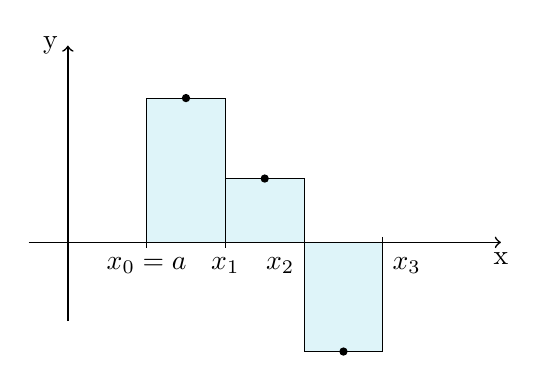
\begin{tikzpicture}[]
		\draw[fill=myblue!30] (1,0) rectangle (2,1.8329); 
		\draw[fill=myblue!30] (2,0) rectangle (3,0.8109);
		\draw[fill=myblue!30] (3,0) rectangle (4,-1.3862);

		\draw[domain=1:3.5] plot [id=rectangular_part_a, samples=100] function { 2*log(4-x) };
		\draw[domain=3.5:5] plot [id=rectangular_part_b, samples=100] function { 2*log(x-3) };
		
		\fill [color=black] (1.5,1.8329) circle (1.5pt);
		\fill [color=black] (2.5,0.8109) circle (1.5pt);
		\fill [color=black] (3.5,-1.3862) circle (1.5pt);
		
		\draw (1,2pt) -- (1,-2pt) node[below] {\(x_0=a\)};
		\draw (2,2pt) -- (2,-2pt) node[below] {\(x_1\)};
		\draw (3,2pt) -- (3,-2pt) node[below left] {\(x_2\)};
		\draw (4,2pt) -- (4,-2pt) node[below right] {\(x_3\)};

		\draw[->,semithick] (-0.5,0) -- (5.5,0) node[below]{x};
		\draw[->,semithick] (0,-1) -- (0,2.5) node[left]{y};

	\end{tikzpicture}
\end{center}

%\todo[inline]{Das letzte Rechteck scheint mir falsch gezeichnet, so stands aber an der Tafel.}
% meiner Ansicht nach korrekt. Entspricht der Rechtecksregel --LH

\begin{definition}[Rechteckregel]
\[ \int\limits_a^b f(x) \,\diff x \mathrel{\dot{=}} \underbrace{\frac{b-a}{n} \cdot\sum_{k=1}^n f(t_k)}_{\text{mittels Rechner auswerten}} \]
\end{definition}

	\item Trapezsummen
	
	\missingfigure{Grafik Trapezfläche}
	
	$h = \frac 1 2 (f_L + f_R)$\\
	$F_\text{Trapez}  = \frac 1 2 (x_R - x_L) (f_L + f_R)$
	
	\missingfigure{Grafik Trapezsumme}
	
	\begin{definition}[Trapezregel]
	\begin{align*}
		\int\limits_a^b f(x) \,\diff x &
		\mathrel{\dot{=}} \frac{b-a}{n}\cdot \frac 1 2 \sum_{k=1}^n \left( f(x_{k-1}) + f(x_k) \right) \\
		&= \frac{b-a}{n} \left(\frac 1 2 \cdot f(a) + \left( \sum_{k=1}^n f(x_k) \right) + \frac 1 2 \cdot f(b) \right) \\
	\end{align*}
	\end{definition}
	
	\begin{note}
		Die Trapezsumme ist für $2 \pi$-periodische Funktionen (z. B. Signalverarbeitung, Fourierentwicklung) die "`beste"' Quadraturformel.
	\end{note}


\end{enumerate}

\subsubsection*{Praxis}
Auswertungsreihe: \( n=8, 16, 32, 64, \ldots \) \newline
vergleiche \( I_8,I_{16}, I_{32}, \ldots\) auf stehende führende Dezimale

\begin{example}
\begin{align*}
	I_8 &= \underline{1},0578 \\
	I_{16} &= \underline{1,2}569 \\
	I_{32} &= \underline{1,24}87 \\
	I_{64} &= \underline{1,249}3 \\
\end{align*}
\end{example}